\chapter{Parallele Algorithmen}

\section{Einleitung}

Indem man Parallelverarbeitung verwendet, kann man sowohl Ressourcen einsparen als auch Ressourcenrestriktionen brechen:
\begin{itemize}
  \item \textbf{Zeitersparnis}: Arbeiten \( p \) Computer an einem Problem, so sind sie bis zu \( p \) mal so schnell.
  \item \textbf{Kommunikationsersparnis}: Fallen Daten verteilt an, so kann man sie auch verteilt (vor)verarbeiten.
  \item \textbf{Energieersparnis}: Zwei Prozessoren mit halber Taktfrequenz brauchen weniger Energie als ein voll getakteter Prozessor.
  \item \textbf{Speicherbeschränkung}: Mehr Prozessoren haben mehr Hauptspeicher, mehr Cache,\dots
\end{itemize}

Es gibt sehr viele Modelle der Parallelverarbeitung, wir werden hier allerdings nur zwei Standardmodelle diskutieren:
\begin{itemize}
  \item \textbf{Prozessornetzwerke mit} \term{Nachrichtenkopplung}\index{Nachrichtenkopplung}.

    Prozessoren sind hier ``normale CPUs'' mit lokalen Speicher. Gemeinsam mit seinem lokalen Speicher wird eine lokale CPU auch \emph{processing element} (PE) genannt. Der Datenaustausch passiert über ein Netzwerk in Form von Nachrichten zwischen zwei Prozessoren.
  \item \textbf{Parallele Registermaschinen mit} \term{Speicherkopplung}\index{Speicherkopplung}.

    Auch hier wird mit normalen CPUs gearbeitet, allerdings haben diese keinen lokalen Speicher, sondern sind über ein Netzwerk mit Speichermodulen verbunden, auf welche alle CPUs zugreifen können. Der Datenaustausch erfolgt über das Netzwerk zwischen einer CPU und einem Speicher.
\end{itemize}

Auf nachrichtengekoppelte Rechner werden wir genauer eingehen.

\begin{figure}[H]
  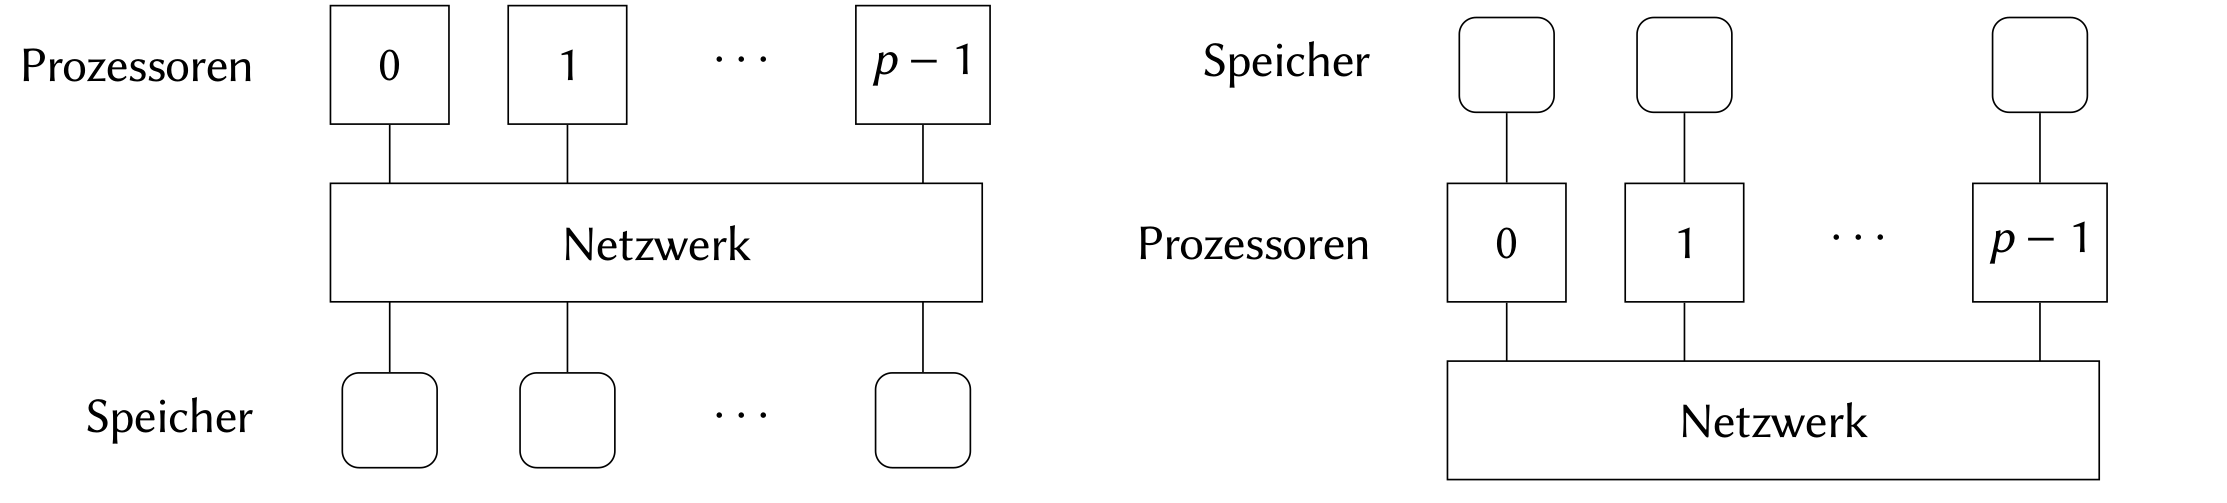
\includegraphics[width=0.9\textwidth]{ParallelArchitectures}
  \caption{Vergleich zwischen \emph{parallelen Registermaschinen mit Speicherkopplung} (links) und einem \emph{Prozessornetzwerk mit Nachrichtenkopplung} (rechts)}
\end{figure}

\subsection{Nachrichtenkopplung vs. Speicherkopplung}

Neben den oben erläuterten Vorteilen von Parallelverarbeitung haben beide Modelle auch Nachteile:

\begin{itemize}
  \item \textbf{Nachrichtenkopplung}:
  \begin{itemize}
    \item Zwei Prozessoren werden zum Datentransport benötigt. Das passt dem Empfänger nicht immer.
    \item Parallelismus muss explizit programmiert werden.
  \end{itemize}
  \item \textbf{Speicherkopplung}:
  \begin{itemize}
    \item \emph{Skalierbarkeit}: Ist eine große Anzahl an Prozessoren sinnvoll?
    \item \emph{Kostenmaß} bei Speicherzugriffskonflikten?
  \end{itemize}
\end{itemize}

Als eine gute Strategie hat es sich erwiesen, den Entwurf für einen verteilten Speicher durchzuführen, da dieser einen viel breiteren Bereich abdecken kann. Die Implementierung erfolgt dann gegebenenfalls für einen gemeinsamen Speicher.

\section{Nachrichtengekoppelte Parallelrechner}

\subsection{Modell}

\begin{itemize}
  \item \textbf{Netzwerk}: Vollständig verknüpftes Punkt-zu-Punkt-Netzwerk
  \begin{itemize}
    \item voll-duplex
    \item Nachrichten überholen sich nicht
  \end{itemize}
  \item \textbf{Prozessoren}: können jeweils maximal gleichzeitig
  \begin{itemize}
    \item eine Nachricht an einen beliebigen Empfänger senden (send(smsg,to))
    \item eine Nachricht von einem beliebigen Sender empfangen (rmsg \( \coloneqq \) recv(from))
    \item \emph{oder} beides gleichzeitig (rmsg \( \coloneqq \) sendRecv(smsg, to, from))
  \end{itemize}
\end{itemize}

Als \emph{Kostenmodell} für das Senden oder Empfangen von \( l \) Bytes verwenden wir
\begin{equation*}
  T_\text{comm}(l) = T_\text{start} + l*T_\text{byte}\text{,}
\end{equation*}
wobei in der Praxis meist \( T_\text{byte} \ll T_\text{start} \). Ignoriert wird hier unter anderem der ``Abstand'' zwischen Sender und Empfänger.

Als \emph{Programmiermodell} verwenden wir \term{SPMD}\index{SPMD} (\emph{single program multiple data}). Alle PEs führen hier dasselbe Programm aus, unterschieden wird lediglich durch ``Ränge'' der PEs (paarweise verschiedene PE-Nummern).

\subsection{Parallele Reduktion}

Im Folgenden gehen wir über die grundlegenden Werkzeuge, die wir benötigen, um parallele Programme analysieren zu können.

\begin{definition}[Reduktion]
  Sei \( \otimes \) eine binäre, assoziative Operation auf einer Menge \( M \).

  Für \( x = (x_0,\dots,x_{p-1}) \in M \) definieren wir
  \begin{equation*}
    R_\otimes(x) = \bigotimes_{i < p}x_i = x_0 \otimes \cdots \otimes x_{p-1}\text{.}
  \end{equation*}
\end{definition}

Nun gilt folgender Satz:

\begin{theorem}
  Wenn \( \otimes \) eine binäre, assoziative Operation ist und \( p \) Elemente \( x_0,\dots,x_{p-1} \) auf \( p \) PEs verteilt sind, dann kann man \( \bigotimes_{i < p}x_i \) in Zeit \( O(\log p) \) auf PE \( 0 \) berechnen.
\end{theorem}

\begin{figure}[H]
  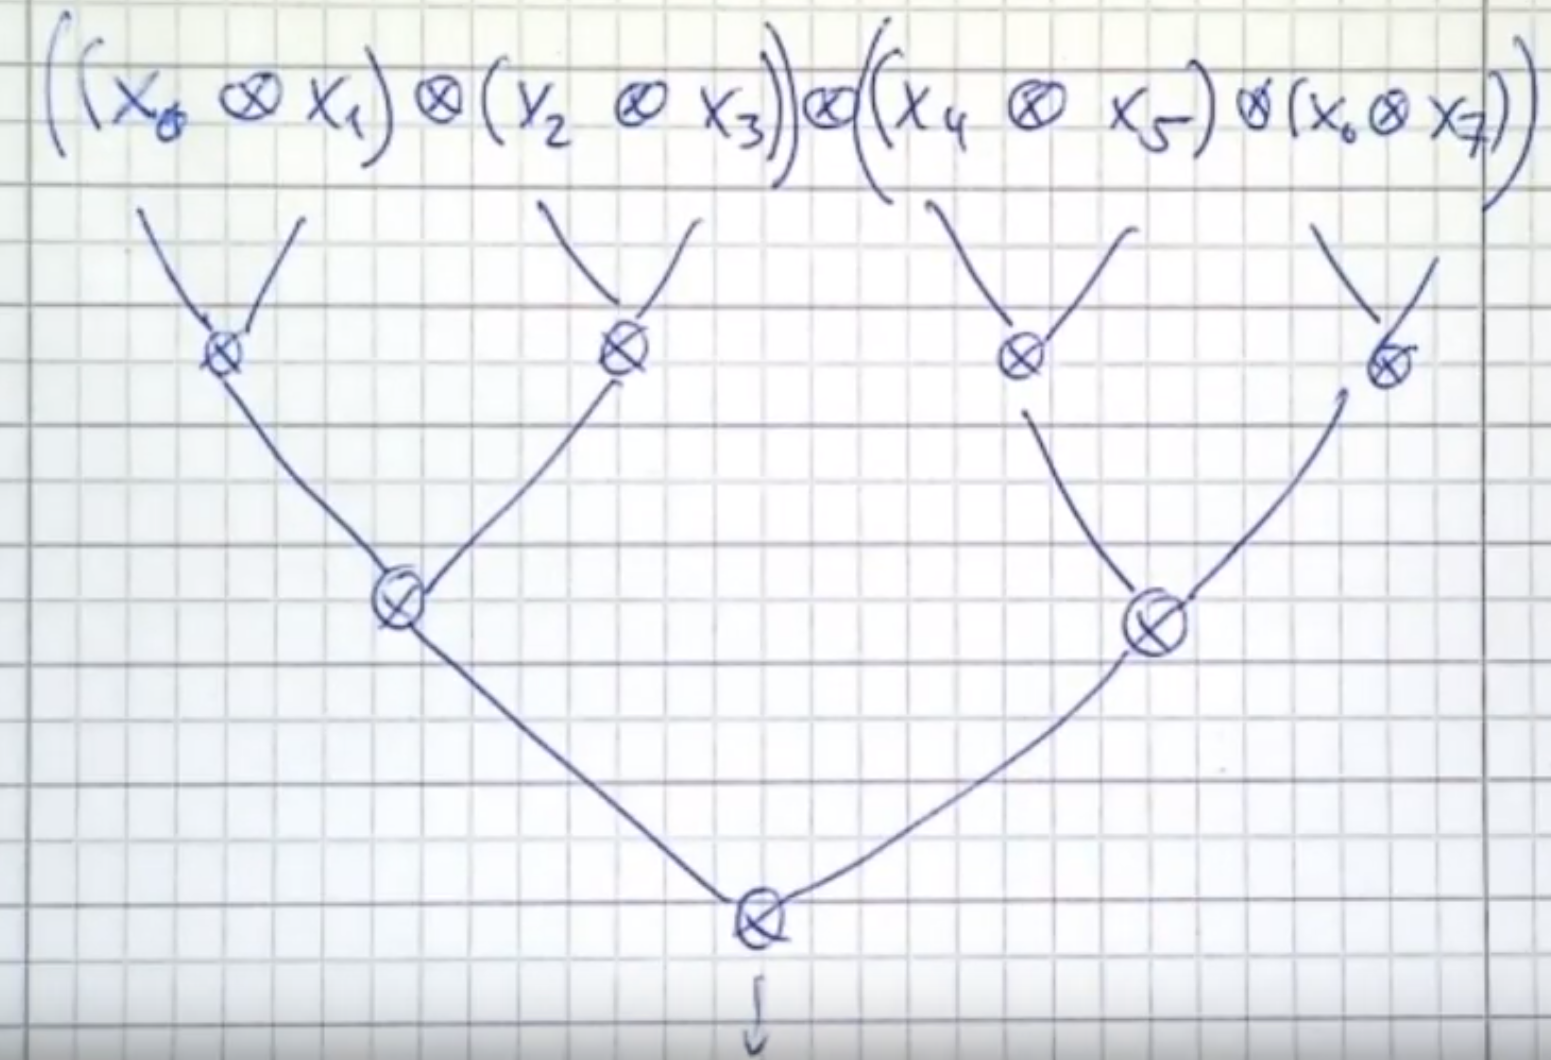
\includegraphics[width=0.6\textwidth]{parallelExecution}
  \caption{Idee hinter obigem Satz}
\end{figure}

Sequenziell wäre die optimale Laufzeit \( O(n) \) gewesen. Auf \( p = n \) PEs hätte man nach obigem Satz eine Laufzeit von \( O(\log n) \) erreicht, also eine Beschleunigung von \( O\left( \frac{n}{\log n} \right) \). ``Ideal'' wäre eine Beschleunigung von \( O(p) = O(n) \) gewesen.

Wie kann man die Beschleunigung noch weiter verbessern?

\subsection{Parallele Reduktion mit \( p < n \)}

Verwenden wir nun \( p < n \) viele PEs, um eine Reduktion auf \( n \) Elementen durchzuführen, so erhält jedes PE \( n/p \) Datenelemente. Die PEs berechnen zuerst die Reduktion der lokalen Elemente, und anschließend wird auf diesen Reduktionen eine parallele Reduktion durchgeführt.
Laufzeit hierfür ist \( O(n/p) + O(\log p) \) und die Beschleunigung somit
\begin{equation*}
  \frac{O(n)}{O(n/p + \log p)}\text{.}
\end{equation*}
Ist \( p \in O(n/\log n) \), so ist die Beschleunigung \( O(p) \).

Man kann also durch Verringerung der Prozessorzahl \( p \) die Beschleunigung in die Nähe von \( p \) bringen. Dieses Prinzip nennt man \term{Brent's Prinzip}\index{Brent's Prinzip}.

\subsection{Analyse paralleler Programme}

Wir interessieren uns in erster Linie für
\begin{itemize}
  \item Laufzeit,
  \item Beschleunigung und
  \item verrichtete Arbeit.
\end{itemize}

Es ist
\begin{itemize}
  \item \( T_\text{par}(I,p) \) die parallele Laufzeit der Probleminstanz \( I \), bearbeitet mit \( p \) PEs,
  \item \( T_\text{seq}(I) \) die sequenzielle Laufzeit der Probleminstanz \( I \) mit dem ``besten bekannten Algorithmus''.
\end{itemize}

Im Allgemeinen ist \( T_\text{seq}(I) < T_\text{par}(I,1) \). Man erhält aber leicht Gleichheit, indem man den parallelen Algorithmus einfach den sequenziellen ausführen lässt, falls nur ein PE zur Verfügung steht.

\begin{definition}[Speedup]
  Wir definieren den \term{Speedup}\index{Speedup} als
  \begin{equation*}
    S(I,p) = \frac{T_\text{seq}(I)}{T_\text{par}(I,p)}\text{.}
  \end{equation*}
  Vergröbert:
  \begin{equation*}
    S(n,p) = \inf\left \{ S(I,p) : n = \left\vert I \right\vert \right \}\text{.}
  \end{equation*}
\end{definition}

Zur Berechnung des Speedups können wir praktischerweise folgende Spezialfälle benutzen, die für Instanzen \( I \), \( I' \) gleicher Größe \( n \) gelten:
\begin{itemize}
  \item \( T_\text{par}(I,p) = T_\text{par}(I',p) = T_\text{par}(n,p) \),
  \item \( T_\text{seq}(I) = T_\text{seq}(I') = T_\text{seq}(n) \)
\end{itemize}